\begin{task}[credit=6]{K-Means}

Folgender Datensatz besteht aus $8$ Punkten:
\begin{equation}
 \begin{aligned}
&x_1=(2,8), \quad x_2=(2,5),\quad x_3=(1,2), \quad x_4=(5,8),\\
&x_5=(7,3), \quad x_6=(6,4),\quad x_7=(8,4), \quad x_8=(4,7).
 \end{aligned}
\end{equation}

\begin{figure}[h!]
\centering
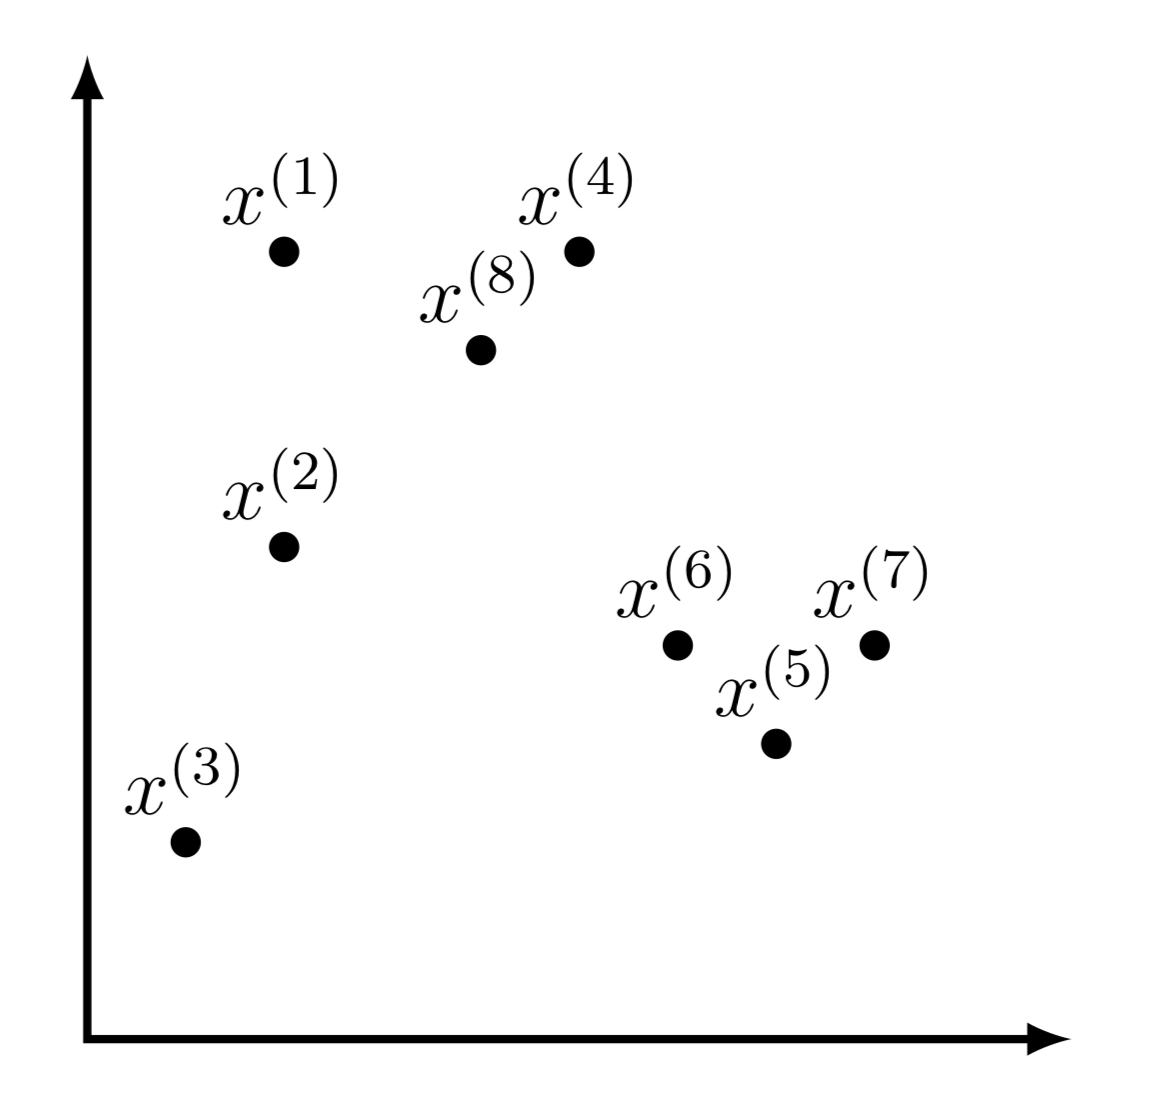
\includegraphics[width=0.4\linewidth]{media/images/kmeans.png}
\caption{Visualisierung des K-Means Datensatzes}
\end{figure}

\begin{subtask}[points=6,title={K-Means Algorithmus}]
Benutzen Sie den K-Means Algorithmus mit der Euklidischen Distanz um diese $8$ Datenpunkte in $K=3$ Cluster einzuteilen.
Nehmen Sie dabei an, dass die Clusterzentren mit den Punkten $x_2$, $x_4$ und $x_8$ initialisiert sind.
Führen Sie zwei Iterationen des K-Means Algorithmus durch und geben Sie die Koordinaten der Zentroide der Cluster an.

\begin{solution}
% Geben sie hier ihre Antwort an.
\end{solution}

\end{subtask}

\end{task}

